\section{Data Visualization in Cultural Heritage}\label{sec:data-visualization-cultural-heritage}

In \Cref{sec:space-time-cube} we were presented with an example of the space-time cube concept in the cultural heritage domain.
Kraak~\citep{kraak2005timelines} showed the paintings collections using this interface with the time slider incorporated in it that allows the
user to choose a time period. There are other visualizations in the cultural heritage domain as well, so in this section, we will present and
discuss some of them.

Nowadays, galleries, libraries, archives, and museums (known as \emph{GLAM} institutions) are in charge of the preservation of cultural
heritage assets~\citep{windhager2018visualization}. When speaking about cultural heritage, we refer to tangible and intangible heritage,
see \Cref{fig:figure2.17}. Tangible includes all the physical assets like historical buildings, artifacts, sculptures, paintings, etc.
Intangible, on the other hand, includes traditions and skills, traditional knowledge, social ceremonies, and others.

\begin{figure}[hbt!]
    \begin{center}
        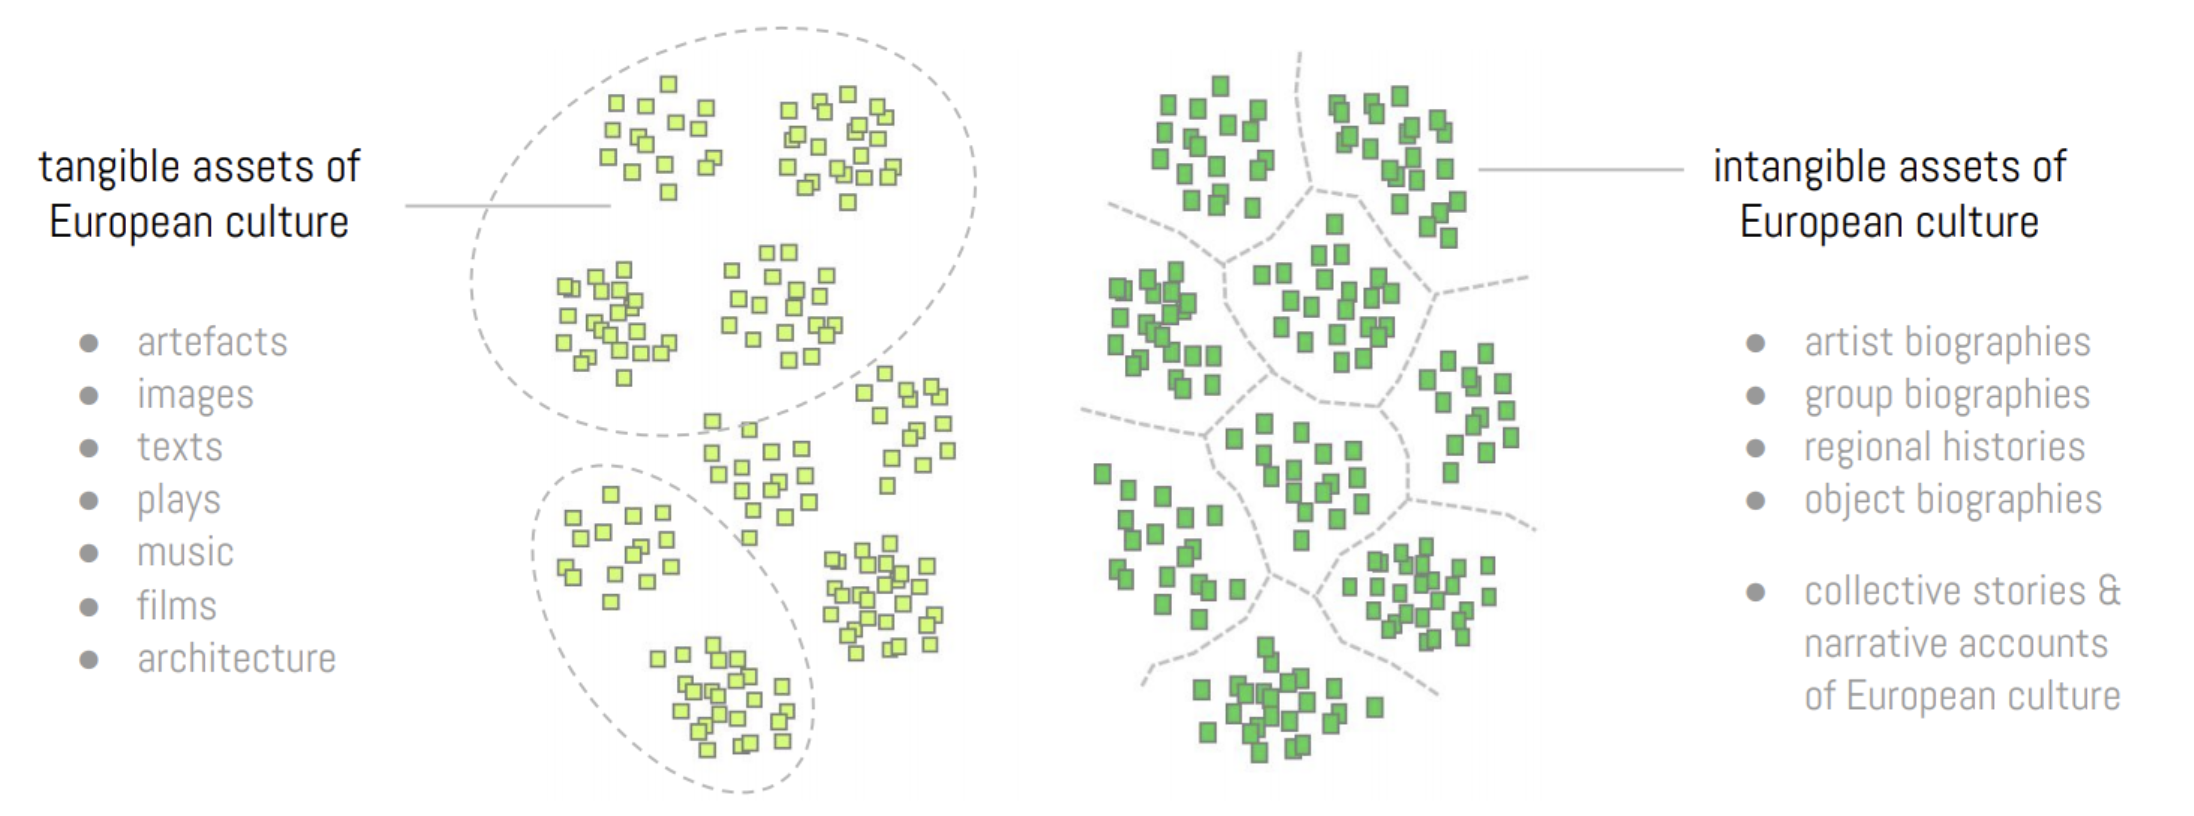
\includegraphics[width=\textwidth]{graphics/2-literature-review/17}
    \end{center}
    \caption{Examples of tangible and intangible assets~\citep{intavia}}
    \label{fig:figure2.17}
\end{figure}

Representing these assets visually by using some kind of interface is a challenging task. One of the main problems is the so-called “museum
fatigue”, where visitors are overwhelmed with the information they see, with computer screens making no exception~\citep{windhager2020many}.
These cultural heritage collections need to be visualized in a way where the most important dimensions of collected data, as seen in
\Cref{fig:figure2.18}, are presented so that the users can easily understand what they are seeing. This is mostly done by combining multiple
visualization types, such as maps with timelines, that allow users to form their own mental model~\citep{windhager2020many}.

\begin{figure}[hbt!]
    \begin{center}
        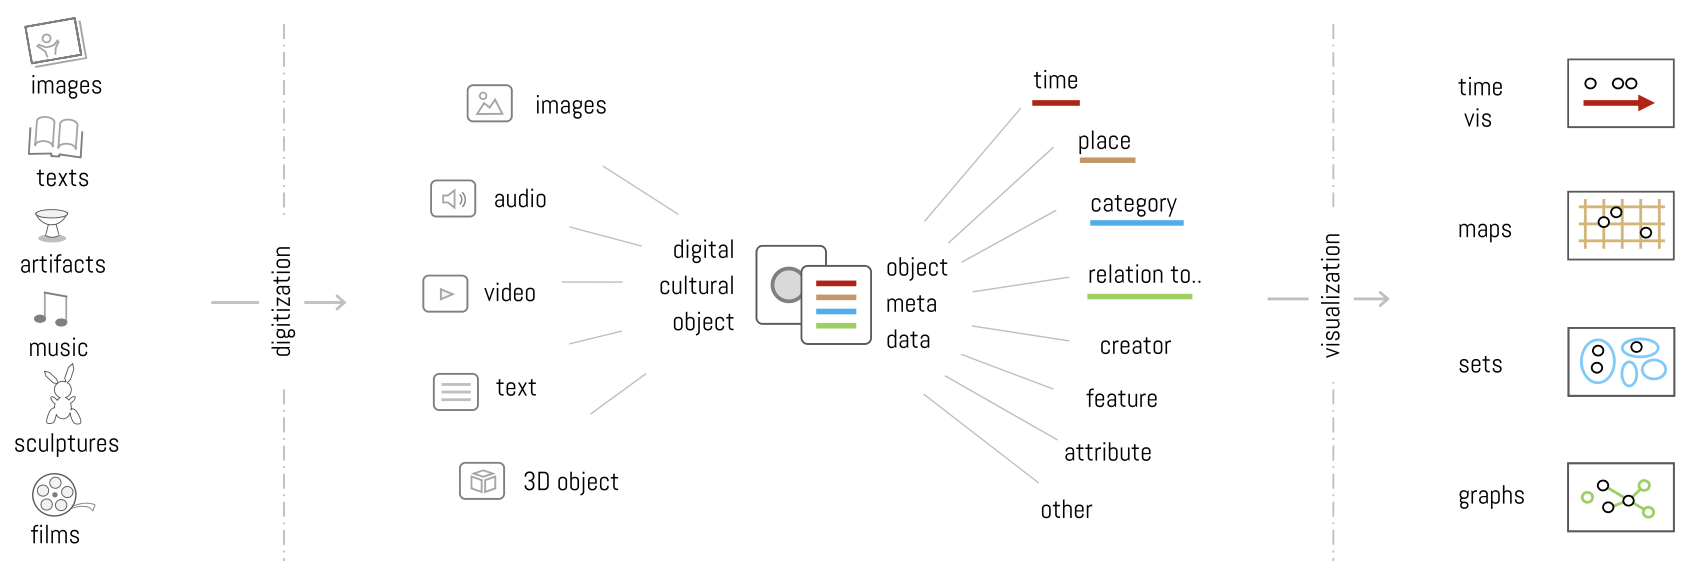
\includegraphics[width=\textwidth]{graphics/2-literature-review/18}
    \end{center}
    \caption{Digitization and visualization of cultural heritage collections~\citep{windhager2020many}}
    \label{fig:figure2.18}
\end{figure}

Now we will discuss a number of data visualization interfaces for cultural heritage collections before shifting our focus to the
visualization of artist biographies that belong to the intangible assets of cultural heritage.

\Cref{fig:figure2.19} shows the interactive timeline explorer by the Google Arts \& Culture~\citep{google} that displays artists in the
selected period. We can choose any artist from the ones shown and read everything related to them as well as explore their artworks.

\clearpage

\begin{figure}[hbt!]
    \begin{center}
        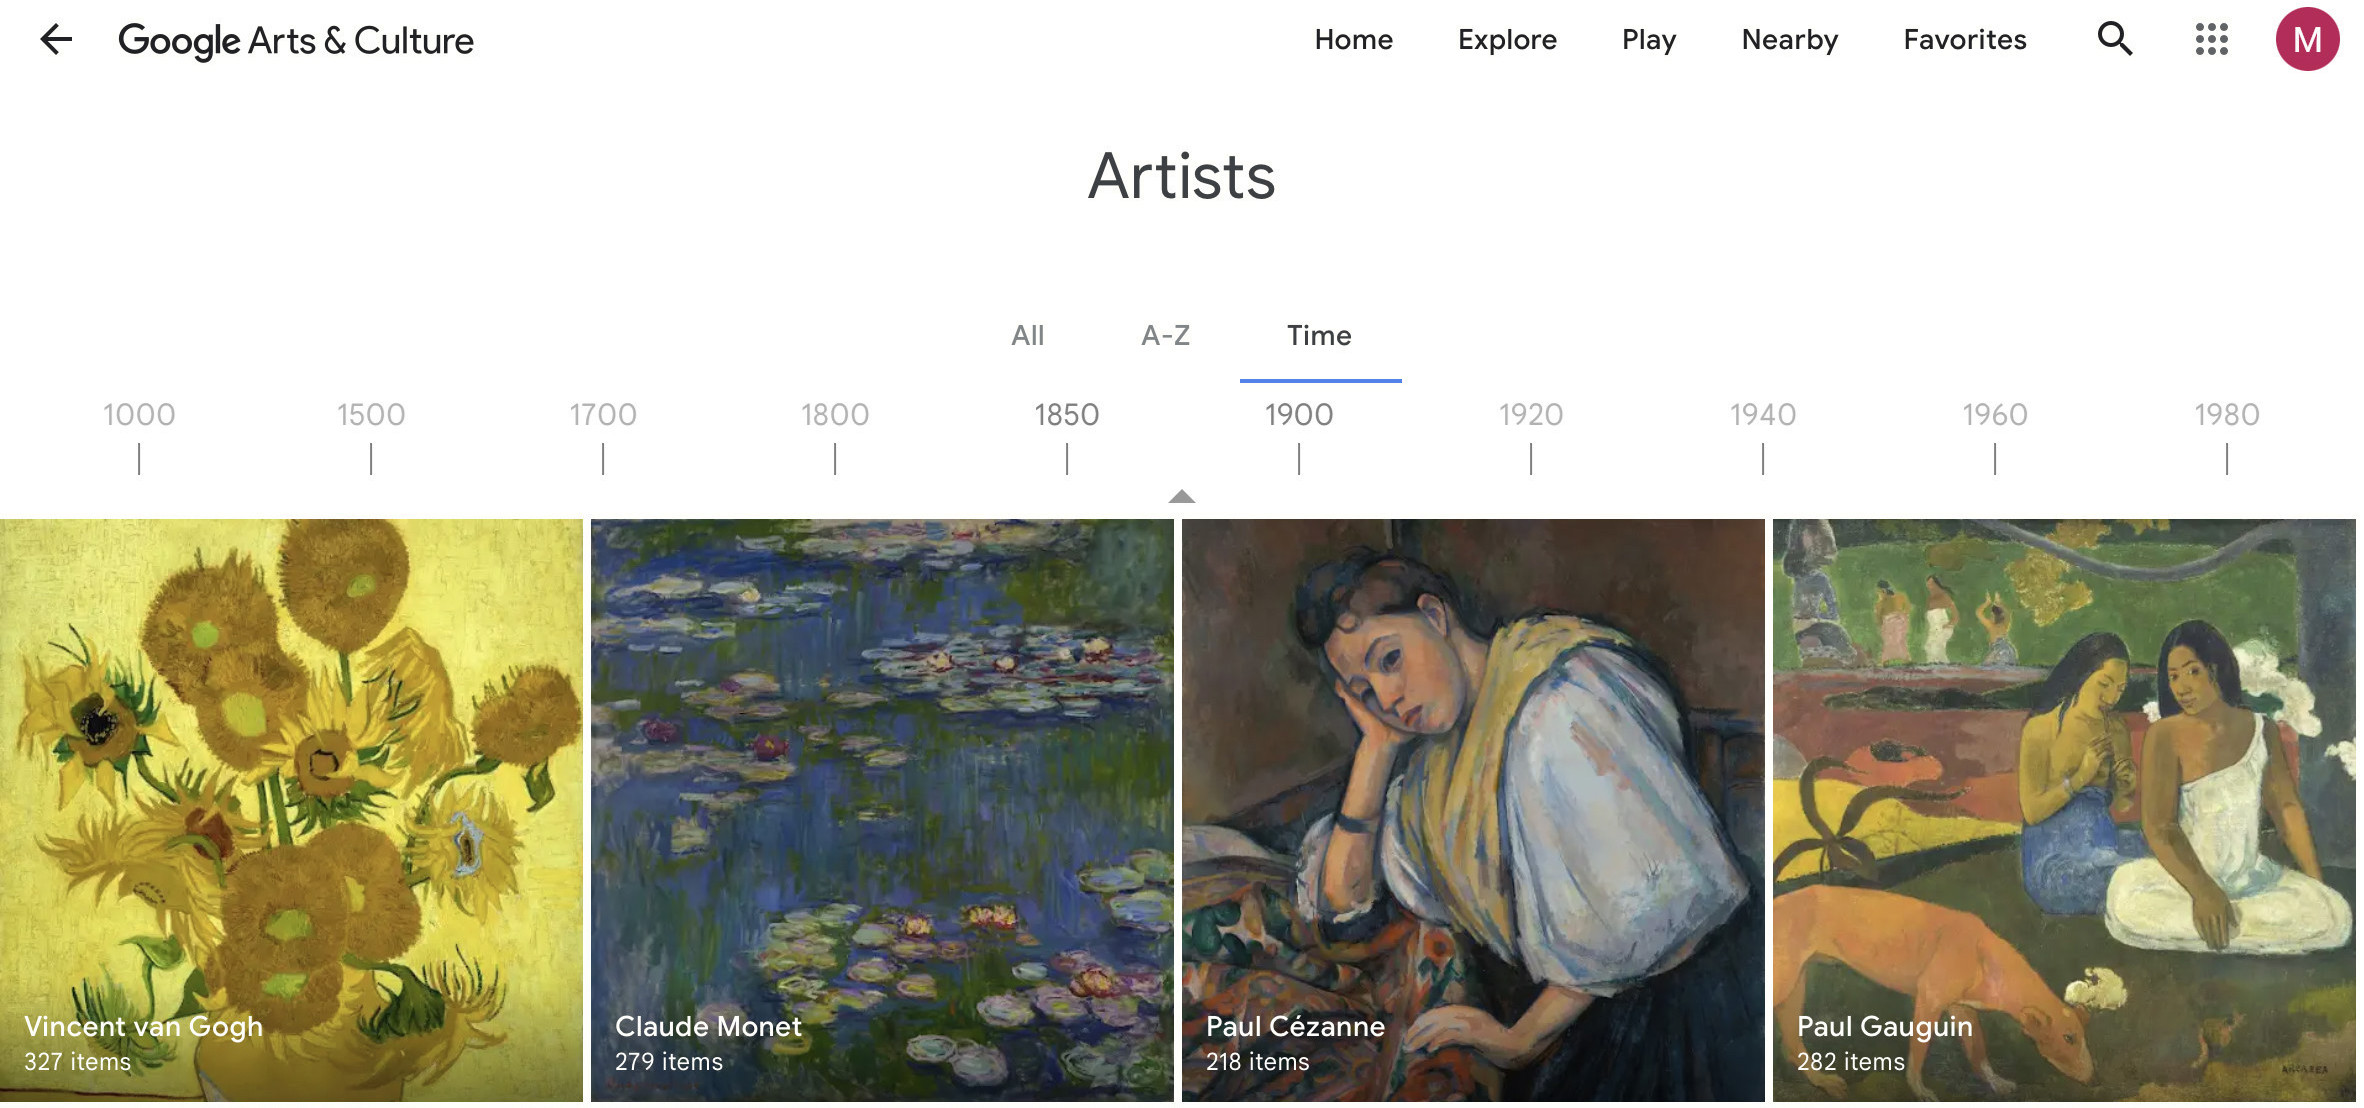
\includegraphics[width=0.95\textwidth]{graphics/2-literature-review/19}
    \end{center}
    \caption{Google Arts \& Culture interactive artists' timeline}
    \label{fig:figure2.19}
\end{figure}

Another similar example is The Museum of the World timeline, a collaboration between the British Museum and
the Google Arts and Culture Lab. Users can explore the museum’s collection by continent, discover connections between objects, filter
the area of interest and see additional information of each object as well~\citep{britishmuseumworld}.

\begin{figure}[hbt!]
    \begin{center}
        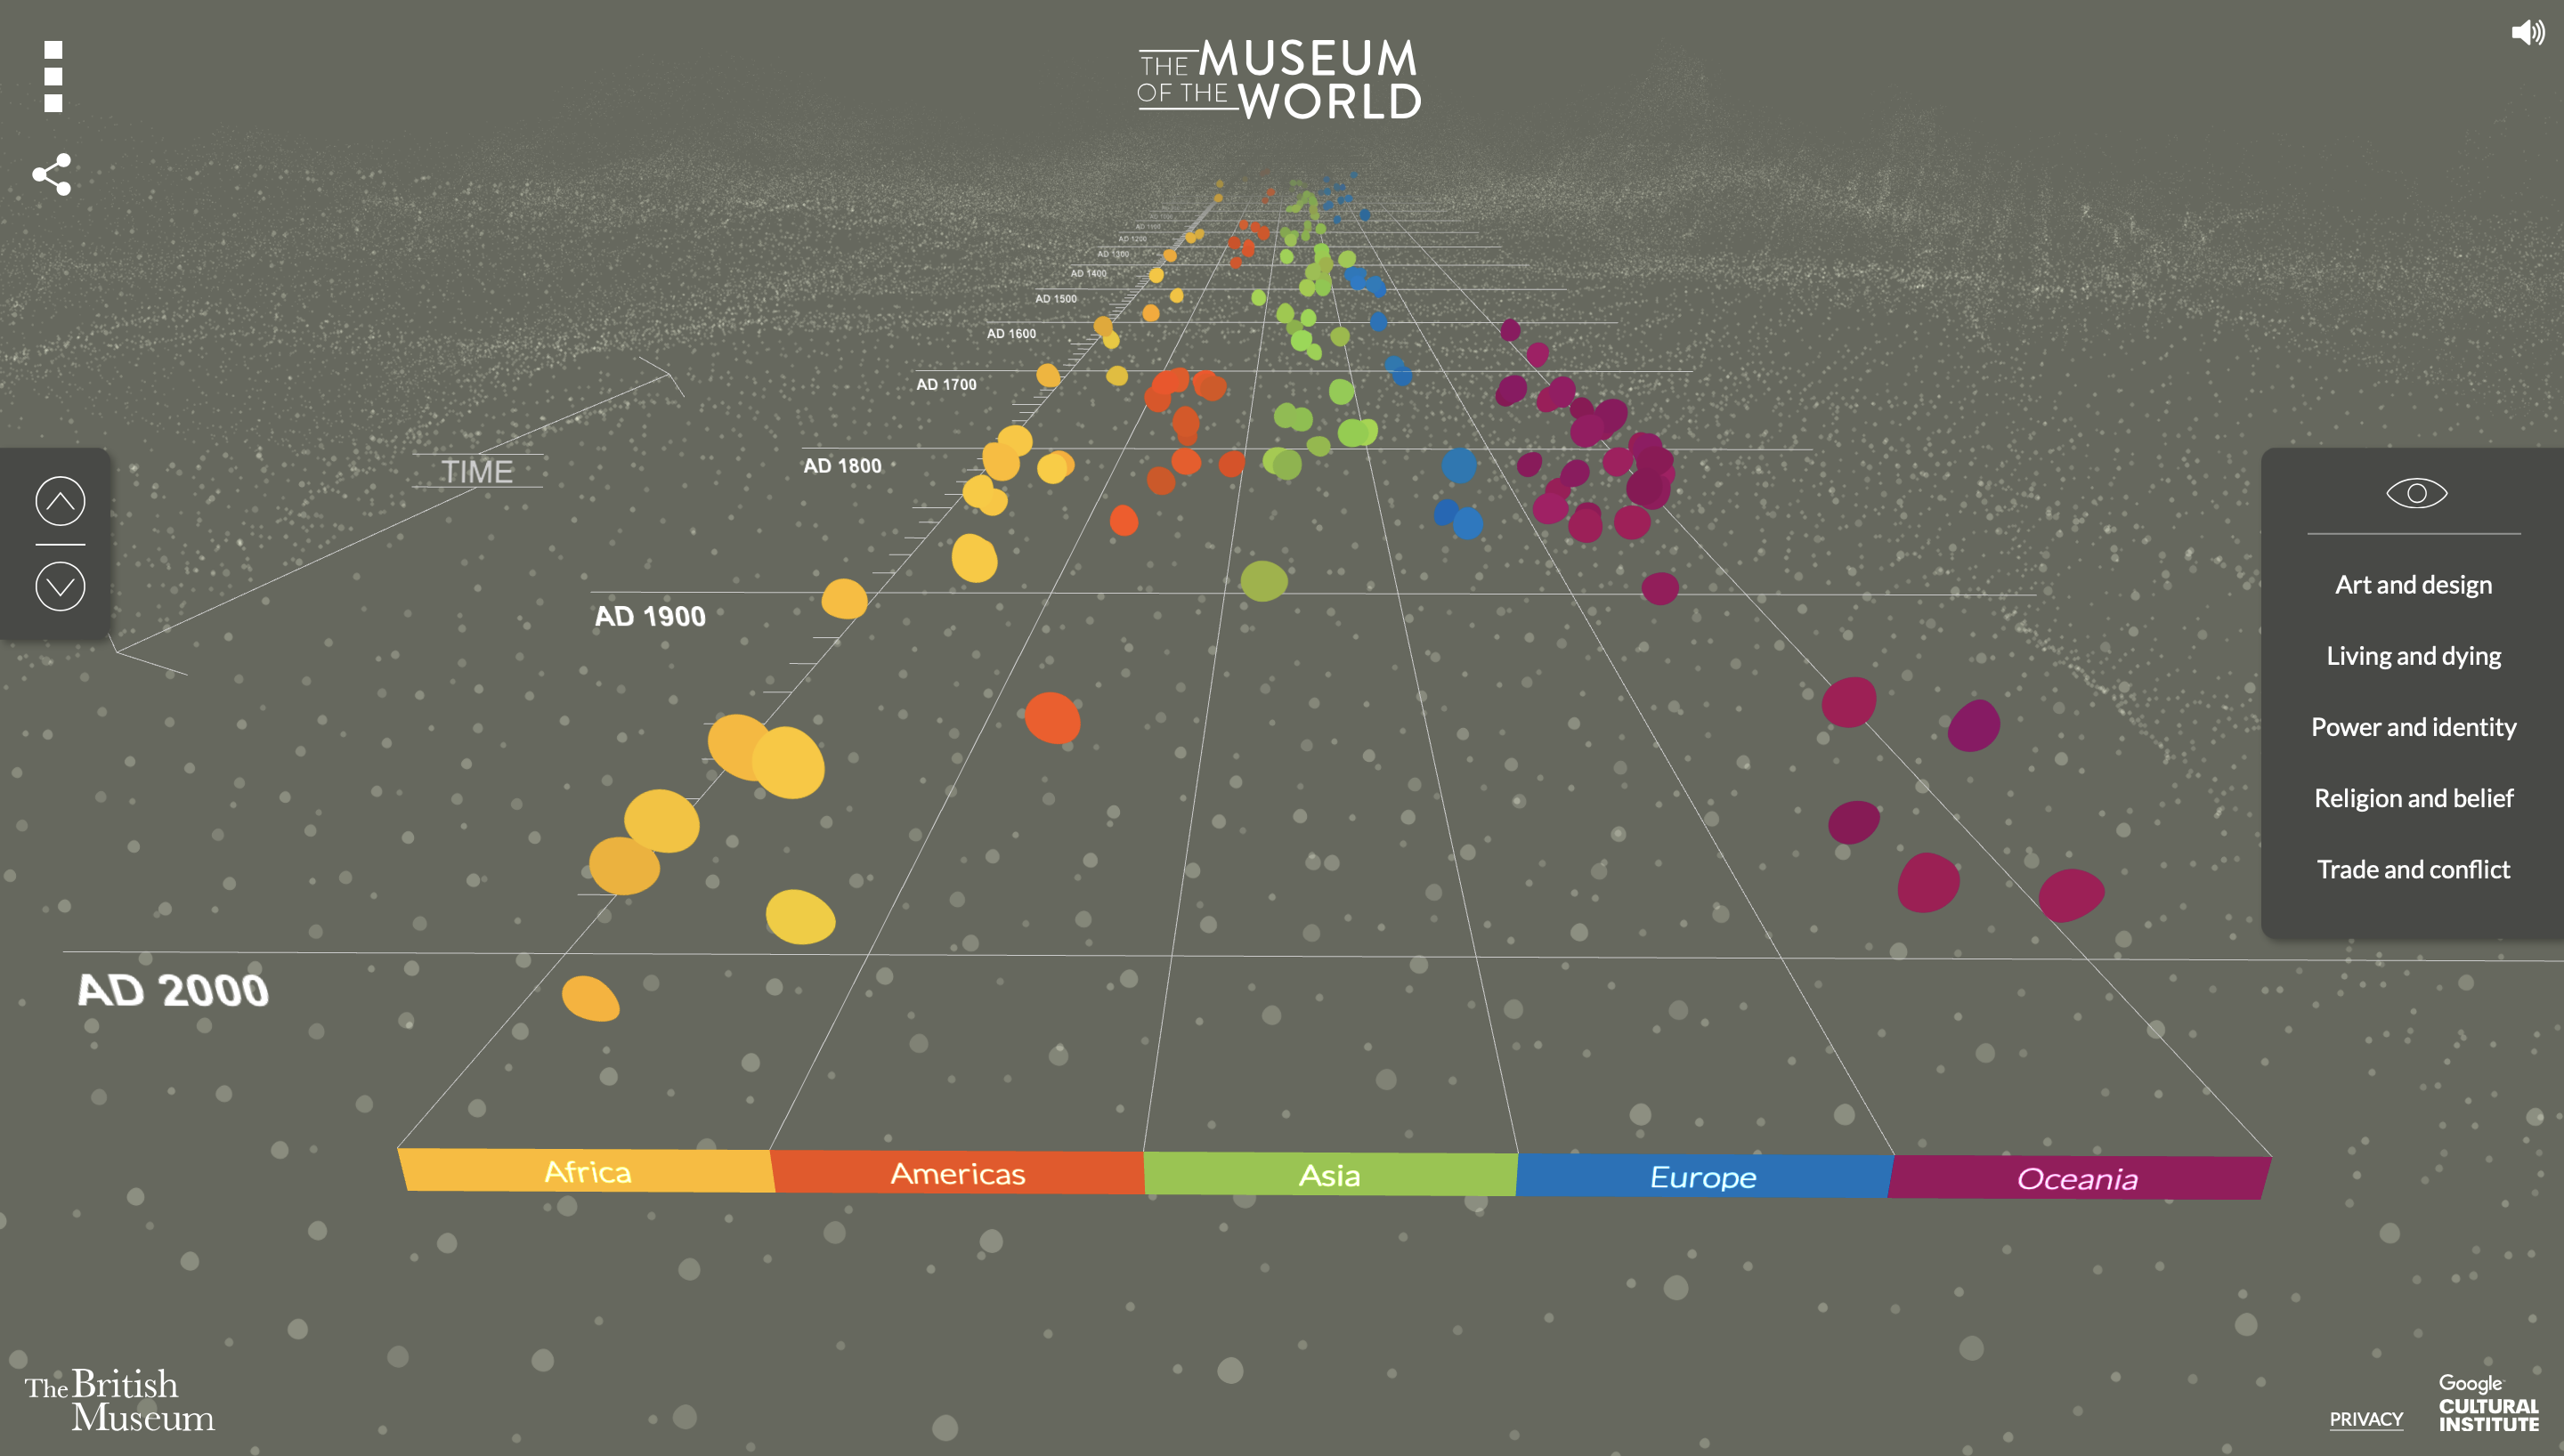
\includegraphics[width=0.95\textwidth]{graphics/2-literature-review/20}
    \end{center}
    \caption{The Museum of the World interactive timeline}
    \label{fig:figure2.20}
\end{figure}

Peripleo by Simon et al.~\citep{simon2016peripleo} is a prototype visualization tool for exploring heterogeneous data through the dimensions
of space and time. Users can search the geographic, temporal, and thematic composition of digital collections, furthermore filtering them to
analyze individual records. The paper provides a detailed description and examples of how to use the tool.

\begin{figure}[hbt!]
    \begin{center}
        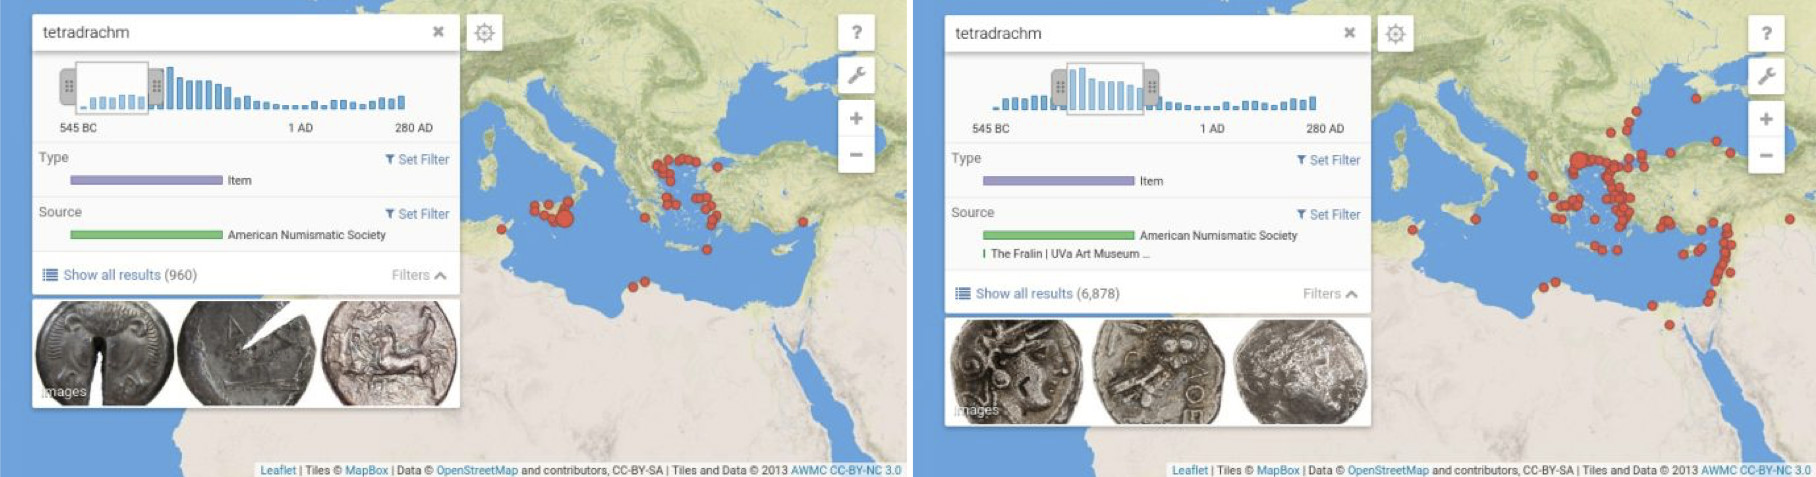
\includegraphics[width=\textwidth]{graphics/2-literature-review/21}
    \end{center}
    \caption{Peripleo tool for exploring digital collections}
    \label{fig:figure2.21}
\end{figure}

Windhager et al.~\citep{windhager2018orchestrating} present the PolyCube interface for visualizing cultural heritage
data. It originates from the space-time cube representation and visualizes large data collections as a wide range of shapes or patterns.
The PolyCube framework incorporates several space-time cubes into a “coordinated multiple cubes” view~\citep{windhager2020many}.

\begin{figure}[hbt!]
    \begin{center}
        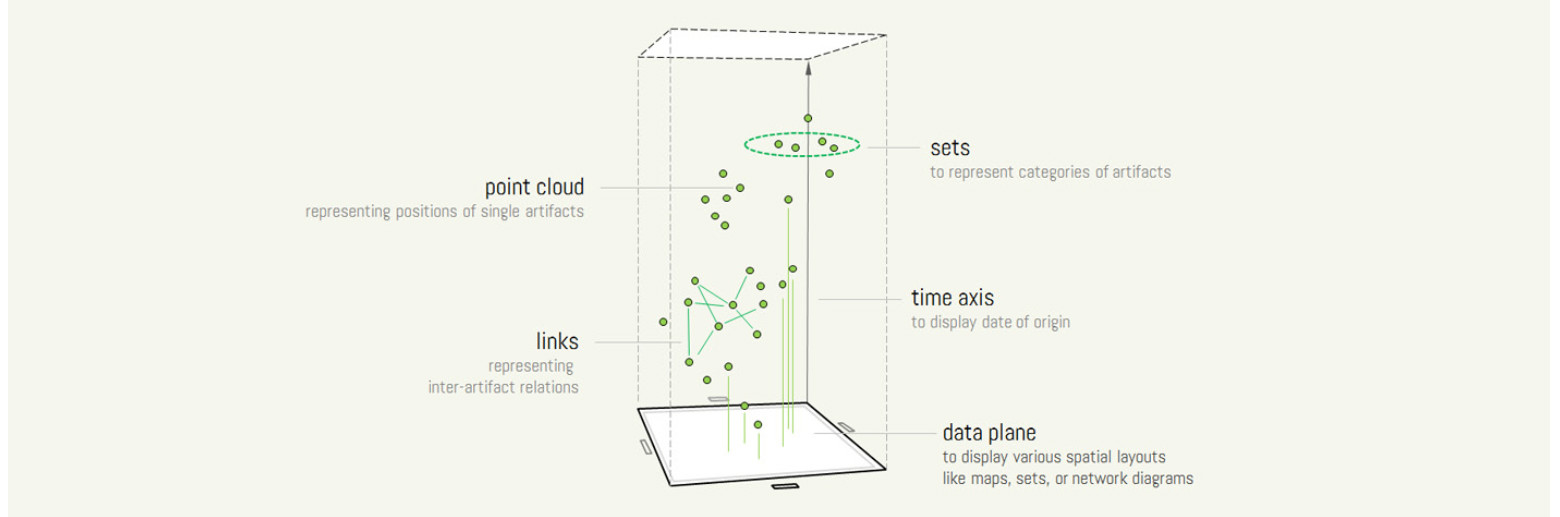
\includegraphics[width=\textwidth]{graphics/2-literature-review/21a}
    \end{center}
    \caption{PolyCube interface for visualizing cultural heritage data}
    \label{fig:figure2.21a}
\end{figure}

We will see an example of the PolyCube framework used to visualize the life and work of an artist in the next section.






